\documentclass[12pt, dvipsnames]{report}

\usepackage{amsmath}
\usepackage{algorithm}
%\usepackage{algorithmic}
\usepackage[noend]{algpseudocode}

\usepackage{amsmath}
\usepackage{amssymb}
\usepackage{amsthm}
\usepackage{amsopn}

\usepackage{kpfonts}

\usepackage{graphicx}

% Probably don't need this on notes anymore
%\usepackage{kbordermatrix}

% Standard tool for drawing diagrams.
\usepackage{tikz}
\usepackage{tkz-berge}
\usepackage{tikz-cd}
\usepackage{tkz-graph}

\usepackage{comment}

%
\usepackage{multicol}

%
\usepackage{framed}

%
\usepackage{mathtools}

%
\usepackage{float}

%
\usepackage{subfig}

%
\usepackage{wrapfig}

%
\let\savewideparen\wideparen
\let\wideparen\relax
\usepackage{mathabx}
\let\wideparen\savewideparen

% Used for generating `enlightening quotes'
\usepackage{epigraph}

% Forget what this is used for :P
\usepackage[utf8]{inputenc}

% Used for generating quotes.
\usepackage{csquotes}

% Allows what to generate links inside
% generated pdf files
\usepackage{hyperref}

% Allows one to customize theorem
% environments in mathematical proofs.
\usepackage{thmtools}

% Gives access to a proof
\usepackage{lplfitch}

% I forget what this is for.
\usepackage{accents}

% A package for drawing simple trees,
% as a substitute for unnesacary TIKZ code
\usepackage{qtree}

% Enables sequent calculus proofs
\usepackage{ebproof}

% For braket notation
\usepackage{braket}

% To change line spacing when using mathematical notations which require some height!
\usepackage{setspace}

%\usepackage[dvipsnames]{xcolor}

\usepackage{float}

% For block commenting
\usepackage{comment}




\setlength\epigraphwidth{8cm}

\usetikzlibrary{arrows, petri, topaths, decorations.markings}

% So you can do calculations in coordinate specifications
\usetikzlibrary{calc}
\usetikzlibrary{angles}

\theoremstyle{plain}
\newtheorem{theorem}{Theorem}[chapter]
\newtheorem{axiom}{Axiom}
\newtheorem{lemma}[theorem]{Lemma}
\newtheorem{corollary}[theorem]{Corollary}
\newtheorem{prop}[theorem]{Proposition}
\newtheorem{exercise}{Exercise}[chapter]
\newtheorem{fact}{Fact}[chapter]

\newtheorem*{example}{Example}
\newtheorem*{proof*}{Proof}

\theoremstyle{remark}
\newtheorem*{exposition}{Exposition}
\newtheorem*{remark}{Remark}
\newtheorem*{remarks}{Remarks}

\theoremstyle{definition}
\newtheorem*{defi}{Definition}

\usepackage{hyperref}
\hypersetup{
    colorlinks = true,
    linkcolor = black,
}

\usepackage{textgreek}

\makeatletter
\renewcommand*\env@matrix[1][*\c@MaxMatrixCols c]{%
  \hskip -\arraycolsep
  \let\@ifnextchar\new@ifnextchar
  \array{#1}}
\makeatother

\renewcommand*\contentsname{\hfill Table Of Contents \hfill}

\newcommand{\optionalsection}[1]{\section[* #1]{(Important) #1}}
\newcommand{\deriv}[3]{\left. \frac{\partial #1}{\partial #2} \right|_{#3}} % partial derivative involving numerator and denominator.
\newcommand{\lcm}{\operatorname{lcm}}
\newcommand{\im}{\operatorname{im}}
\newcommand{\bint}{\mathbf{Z}}
\newcommand{\gen}[1]{\langle #1 \rangle}

\newcommand{\End}{\operatorname{End}}
\newcommand{\Mor}{\operatorname{Mor}}
\newcommand{\Id}{\operatorname{id}}
\newcommand{\visspace}{\text{\textvisiblespace}}
\newcommand{\Gal}{\text{Gal}}

\newcommand{\xor}{\oplus}
\newcommand{\ft}{\wedge}
\newcommand{\ift}{\vee}

\newcommand{\prob}{\mathbf{P}}
\newcommand{\expect}{\mathbf{E}}
\DeclareMathOperator{\Var}{\mathbf{V}}
\newcommand{\Ber}{\text{Ber}}
\newcommand{\Bin}{\text{Bin}}

%\newcommand{\widecheck}[1]{{#1}^{\ft}}

\DeclareMathOperator{\diam}{\text{diam}}

\DeclareMathOperator{\QQ}{\mathbf{Q}}
\DeclareMathOperator{\ZZ}{\mathbf{Z}}
\DeclareMathOperator{\RR}{\mathbf{R}}
\DeclareMathOperator{\HH}{\mathbf{H}}
\DeclareMathOperator{\CC}{\mathbf{C}}
\DeclareMathOperator{\AB}{\mathbf{A}}
\DeclareMathOperator{\PP}{\mathbf{P}}
\DeclareMathOperator{\MM}{\mathbf{M}}
\DeclareMathOperator{\VV}{\mathbf{V}}
\DeclareMathOperator{\TT}{\mathbf{T}}
\DeclareMathOperator{\LL}{\mathcal{L}}
\DeclareMathOperator{\EE}{\mathbf{E}}
\DeclareMathOperator{\NN}{\mathbf{N}}
\DeclareMathOperator{\DQ}{\mathcal{Q}}
\DeclareMathOperator{\IA}{\mathfrak{a}}
\DeclareMathOperator{\IB}{\mathfrak{b}}
\DeclareMathOperator{\IC}{\mathfrak{c}}
\DeclareMathOperator{\IP}{\mathfrak{p}}
\DeclareMathOperator{\IQ}{\mathfrak{q}}
\DeclareMathOperator{\IM}{\mathfrak{m}}
\DeclareMathOperator{\IN}{\mathfrak{n}}
\DeclareMathOperator{\IK}{\mathfrak{k}}
\DeclareMathOperator{\ord}{\text{ord}}
\DeclareMathOperator{\Ker}{\textsf{Ker}}
\DeclareMathOperator{\Coker}{\textsf{Coker}}
\DeclareMathOperator{\emphcoker}{\emph{coker}}
\DeclareMathOperator{\pp}{\partial}
\DeclareMathOperator{\tr}{\text{tr}}

\DeclareMathOperator{\supp}{\text{supp}}

\DeclareMathOperator{\codim}{\text{codim}}

\DeclareMathOperator{\minkdim}{\dim_{\mathbf{M}}}
\DeclareMathOperator{\hausdim}{\dim_{\mathbf{H}}}
\DeclareMathOperator{\lowminkdim}{\underline{\dim}_{\mathbf{M}}}
\DeclareMathOperator{\upminkdim}{\overline{\dim}_{\mathbf{M}}}
\DeclareMathOperator{\lhdim}{\underline{\dim}_{\mathbf{M}}}
\DeclareMathOperator{\lmbdim}{\underline{\dim}_{\mathbf{MB}}}
\DeclareMathOperator{\packdim}{\text{dim}_{\mathbf{P}}}
\DeclareMathOperator{\fordim}{\dim_{\mathbf{F}}}

\DeclareMathOperator*{\argmax}{arg\,max}
\DeclareMathOperator*{\argmin}{arg\,min}

\DeclareMathOperator{\ssm}{\smallsetminus}

\title{Waves Light and Heat}
\author{Jacob Denson}

\begin{document}

\pagenumbering{gobble}
\maketitle
\tableofcontents
\pagenumbering{arabic}

\chapter{Physical Examples}

\section{Simple Harmonic Motions}

So many physical behaviours can be studied from the perspective of oscillation and vibration. The common feature of this phenomenon is \emph{periodicity}, a pattern repeating itself indefinitely. Almost always these oscillations are sinusoidal, because the physical behaviour reduces (at least approximately) to the study of the \emph{simple harmonic oscillator} $\ddot{x} = - \omega_0^2 x$, and it's higher dimension variants, in which the force on an object is proportional to it's spatial displacement from equilibrium. The general solution of such an equation is
%
\[ x = A \sin(\omega_0 t + \phi) = C_1 \sin(\omega_0 t) + C_2 \cos(\omega_0 t). \]
%
The terms in this equation occur so often there are special names reserved for them:
%
\begin{itemize}
    \item $A$ is the \emph{amplitude}.
    \item $\phi$ is the \emph{phase shift} or \emph{phase lag}.
    \item $\omega_0$ is the \emph{angular frequency} of oscillation.
    \item The frequency is then $f = \omega_0 / 2\pi$.
\end{itemize}
%
Note that in the case of simple harmonic motion, the frequency and period of the oscillation is fixed; it is independent of the initial position and velocity of the object.

Most phenomena in physics is \emph{nonlinear}, and thus does not precisely follow simple harmonic oscillation. Nonetheless, simple harmonic oscillation is often a useful approximation of many physical behaviours. Given an arbitrary equation of the form $\ddot{x} = F(x)$ with $F(0) = 0$ and $F'(0) < 0$, solutions to this equation with initial conditions close to the origin, and starting with small velocity are closely approximated by solutions of the equation $\ddot{x} = F'(x_0) x$, which is a simple harmonic oscillation. Let us consider some physical examples of simple harmonic motion:
%
\begin{itemize}
    \item The motion of an object held on a \emph{linear spring} follows \emph{Hooke's Law}
    %
    \[ m \ddot{x} = -k x. \]
    %
    It oscillates at an angular frequency of $\sqrt{k/m}$.

    \item The motion of a pendulum of length $l$, if $\theta$ denotes the angle of the pendulum relative to the vertical, and $g$ the gravitational force, follows the equation
    %
    \[ \ddot{\theta} = - (g/l) \sin \theta. \]
    %
    For $|\theta| \ll 1$, we have $\ddot{\theta} \approx - (g/l) \theta$, and thus we expect that, for small angles, the pendulum to oscillate at a frequency of $\sqrt{g/l}$.

    \item Consider a piston of mass $M$ and surface area $A$ holding down a fixed number of $N$ moles of air particles by gravity. Boyle's law tells us that the pressure $P$ pushing up on the lever is equal to $NRT/V$, where $R$ is the ideal gas constant, $T$ is the temperature of the air inside the piston, and $V$ is the volume of the space inside the piston. Now if $H$ is the height of the lever relative to the ground, then $V = AH$. If we assume the force pushing down on the lever is roughly independent of $H$ with some magnitude $F$, i.e. the force do the gravity over short distances, and the atmospheric pressure, then our equation of motion becomes
    %
    \[ M \ddot{H} = A P_{\text{up}} - F = NRT/H - F.  \]
    %
    This is a nonlinear equation in $H$. But near the equilibrium point $H_{\text{eq}} = NRT / F$, the equation behaves approximately like a simple harmonic oscillator. If we let $H_\Delta = H - H_{\text{eq}}$, then we find that for $|H_\Delta| \ll 1$, we have
    %
    \[ M \ddot{H}_\Delta \approx \frac{-NRT}{H_{\text{eq}}^2} H_\Delta = \frac{-F^2}{NRT} H_\Delta. \]
    %
    The piston thus oscillates near $H_{\text{eq}}$ at a frequency of $F / (NRTM)^{1/2}$.
\end{itemize}
%
One useful thing to notice is that simple harmonic motion is just the projection of a point in a plane travelling about a circle of radius $A$ at an angular frequency of $\omega_0$. This is closely related to the \emph{complexification} of the study of oscillation. A general solution of the equation $\dot{x} = - \omega_0^2 x$ over the complex numbers is an equation of the form
%
\[ x = A e^{i (\omega_0 t + \phi)} = C_1 e^{i \omega_0 t} + C_2 e^{-i \omega_0 t}. \]
%
Since our differential equation is linear, with real coefficients, the real and imaginary parts of any complex solution will be a real solution, so there is really no more generality in the study of complex solutions. They are just a notational convenience.

\section{Superposition}

Another useful tool in the study of linear oscillators is the principle of \emph{superposition}, i.e. that the linear combination of solutions to the equation is a solution. One solution of the harmonic oscillator is $x = \cos(\omega_0 t)$, with $x_0 = 1$, and $\dot{x}_0 = 0$. Another solution is $x = \omega_0^{-1} \sin(\omega_0 t)$, with $x_0 = 0$, and $\dot{x}_0 = 1$. The principle of superposition tells us that the general solution of the harmonic oscillator with initial conditions $x_0$ and $\dot{x}_0$ is
%
\[ x = x_0 \cos(\omega_0 t) + \frac{\dot{x}_0}{\omega_0} \sin(\omega_0 t). \]
%
Let us dwell on some phenomena which result from the principle of superposition.

We see the phenomenon of \emph{interference}. Namely, the sum of two waves travelling at the same frequency and whose amplitudes have the same sign results in a wave travelling at the same frequency, but with a larger amplitude. Thus we witness \emph{constructive interference}. A simple example of this phenomenon follows from the calculation
%
\[ \sin(t) + \sin(t + \phi) = (1 + \cos(\phi)) \sin(t) + \sin(\phi) \sin(t + \pi/2). \]
%
For $\phi = 0$, we get
%
\[ \sin(t) + \sin(t) = 2 \sin(t), \]
%
i.e. a wave travelling at twice the amplitude of the two original waves, so we see constructive interference. If $\phi = \pi$, then we find that
%
\[ \sin(t) + \sin(t + \pi) = 0, \]
%
i.e. the waves perfectly cancel one another out, and we get deconstructive interference. One may witness this phenomenon if we consider a microphone placed between two speakers playing the same sound at the same time. The microphone will then hear that sound at twice the volume. On the other hand, if we move the speaker closer to one speaker than the other, then the phase difference of the two speakers relative to the microphone changes, with one speaker eventually cancelling the other out.

We can also consider the superposition of $N+1$ waves travelling at the same frequency but with regularly spaced phase delay. Thus we consider
%
\[ \sum_{k = 0}^{N-1} \sin(\omega_0 t + k \delta). \]
%
This is the imaginary part of the sum of the $N$ vectors
%
\[ X = \sum_{k = 0}^{N-1} e^{i (\omega_0 t + k \delta)} = \sum_{k = 0}^{N-1} X_k. \]
%
Note that the points $\{ X_0, \dots, X_{N-1} \}$ forms consecutive vertices of a polygon. Consider the unit vector $X_A$ whose angle is equal to the average angle of the vectors $\{ X_k \}$, i.e.
%
\[ \frac{1}{N} \sum_{k = 0}^{N-1} (\omega_0 t + k \delta) = \omega_0 t + \frac{N-1}{2} \delta. \]
%
For $0 \leq i < (N-1)/2$, each of the vectors $X_i + X_{N-i-1}$ lies in the direction of $X_A$, and if $N$ is odd, then $X_{(N-1)/2} = X_A$. Thus the sum must also point in the direction of $X_A$. The magnitude clearly does not depend on $\omega_0$, so we may as well calculate the magnitude of
%
\[ \left| \sum_{k = 0}^{N-1} e^{i k \delta} \right| = \frac{|e^{N i \delta} - 1|}{|e^{i \delta} - 1|} = \frac{2 \sin(N \delta /2)}{2 \sin(\delta / 2)} = \frac{\sin(N\delta/2)}{\sin(\delta/2)}. \]
%
Thus we conclude that
%
\[ X = \frac{\sin(N\delta/2)}{\sin(\delta/2)} X_A, \]
%
thus
%
\[ \sum_{k = 0}^{N-1} \sin(\omega_0 t + k \delta) = \frac{\sin(N\delta/2)}{\sin(\delta/2)} \sin \left( \omega_0 t + \frac{N-1}{2} \delta \right). \]
%
For $\delta \ll 1/N$, we have
%
\[ \frac{\sin(N \delta/2)}{\sin(\delta/2)} \approx N - \frac{N (N + 1)(N - 1)}{24} \delta^2 + O( (N \delta)^3 ) \]
%
Thus the amplitude of the overall sum is proportional to $N$. However, as $\delta$ increases beyond this range the deconstructive interference between the different phases causes the overall amplitude to decrease, up to when $\delta = 2\pi / N$, in which case we have complete cancellation of all phases.

We also have the phenomenon of \emph{beats}. Consider the cosine addition law
%
\[ \cos(a) + \cos(b) = 2 \cos \left( \frac{a + b}{2} \right) \cos \left( \frac{a - b}{2} \right). \]
%
This tells us, for instance, that
%
\[ \cos(\omega_1 t) + \cos(\omega_2 t) = 2 \cos \left( \left( \frac{\omega_1 + \omega_2}{2} \right) t \right) \cos \left( \left( \frac{\omega_1 - \omega_2}{2} \right) t \right). \]
%
If $|\omega_1 - \omega_2| \ll \omega_1 + \omega_2$, then the sum will roughly behave like these waves at twice the amplitude, modulated by a low frequency signal.
%
\begin{center}
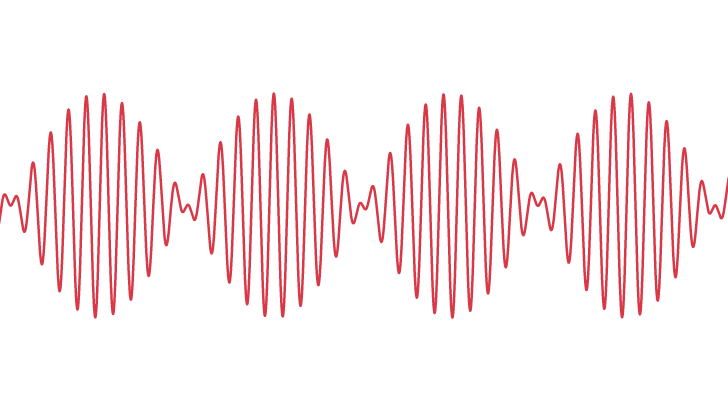
\includegraphics[width=0.5\textwidth]{beats.png}
\end{center}
%
If one were to place two tuning forks together vibrating at the same amplitude, and frequencies 300 and 302 Hertz, then one would hear a wave with twice the amplitude and with frequency 301 Hertz, but modulated by a signal travelling at 1 Hertz.

\section{Dampening}

Now consider the \emph{damped} harmonic oscillator
%
\[ \ddot{x} = -\omega_0^2 x - b \dot{x}. \]
%
The values $\xi \in \CC$ that produce a solution $x = e^{i \xi x}$ to this equation satisfies $\xi^2 = \omega_0^2 + ib \xi$, so that
% xi^2 - ibxi - k
\[ \xi = \frac{ib}{2} \pm \sqrt{\omega_0^2 - b^2/4}. \]
%
Provided that the oscillator $b < 2 \omega_0$, so that the equation is \emph{lightly damped}, we see that solutions to this equation are of the form
%
\[ x = A e^{- (b/2) t} \cos(\omega_1 t + \phi), \]
%
where solutions continue to oscillate at an angular frequency of
%
\[ \omega_1 = \sqrt{\omega_0^2 - b^2 / 4}, \]
%
slightly smaller than the frequency if there was no dampening, but now also with a exponential dampening factor of $e^{-(b/2)t}$. On the other hand, if $b > 2 \omega_0$, so the oscillation is \emph{over damped}, then the solutions to the equation are of the form $x = c_1 e^{-\delta_1 t} + c_2 e^{-\delta_2 t}$, where $0 < \delta_1, \delta_2 < b/2$ are solutions to the equation
%
\[ \delta = b/2 \pm \sqrt{b^2 / 4 - \omega_2}. \]
%
In particular, at the \emph{critical damping point} with $b = 2 \omega_0$, the solution is $x = (c_1 + c_2 t) e^{- (b/2) t}$, which is the amount of damping which results in the fastest return to equilibrium.

On the other hand, now let us add a \emph{driving force}, i.e. consider the harmonic oscillator
%
\[ \ddot{x} = F_D(t) - \omega_0^2 x - b\dot{x}, \]
%
for some fixed driving force $F_D$. Let us consider a simple driving force, e.g. $F_D(t) = \cos(\omega_D t)$. It is \emph{only} a frequency of $\omega_D$ that is being added over time, whereas the dampening force causes all frequencies to decay over time. Thus we might expect that if this equation has a \emph{steady state solution}, i.e. a solution to which other solutions decay over time, then we might expect this solution to oscillate at a frequency $\omega_D$. If we consider a function of the form $x(t) = A \cos(\omega_D t + \phi)$, then the equation becomes
%
\[ A (\omega_0^2 - \omega_D^2) \cos(\omega_D t + \phi) = \cos(\omega_D t) + b \omega_D A \sin(\omega_D t + \phi). \]
%
Using the addition formulas for cosine and sine, and the independence of the functions $t \mapsto \cos(\omega_D t)$ and $t \mapsto \sin(\omega_D t)$, we conclude that we must have
%
\[ A [(\omega_0^2 - \omega_D^2) \cos(\phi) - b \omega_D \sin(\phi)] = 1 \]
%
and
%
\[ A [b \omega_D \cos(\phi) + (\omega_0^2 - \omega_D^2) \sin(\phi)] = 0 \]
%
Since $A = 0$ does not give a solution to the problem, we must have $A \neq 0$, and so we conclude that
%
\[ b \omega_D \cos(\phi) + (\omega_0^2 - \omega_D^2) \sin(\phi) = 0. \]
%
This means that there exists $\lambda \neq 0$ such that $\cos(\phi) = \lambda (\omega_0^2 - \omega_D^2)$, and $\sin(\phi) = - \lambda b \omega_D$, where
%
\[ \lambda^2 = \frac{1}{(\omega_0^2 - \omega_D^2)^2 + (b \omega_D)^2} \]
%
In particular,
%
\[ \tan(\phi) = \frac{- b \omega_D}{\omega_0^2 - \omega_D^2}. \]
%
Plugging this into the first equation gives that
%
\[ A = \frac{1}{\lambda} \frac{1}{(\omega_0^2 - \omega_D^2)^2 + (b \omega_D)^2} = \frac{1}{\sqrt{(\omega_0^2 - \omega_D^2)^2 + (b \omega_D)^2}}. \]
%
Thus we have found a steady state solution to the equation. For a fixed $\omega_0$, this steady state will have the highest amplitude when
%
\[ \omega_D = \max \left( 0, \sqrt{\omega_0^2 - b^2/2} \right). \]
%
This is the \emph{resonant frequency} for the equation. The phase lag for the resonant frequency will satisfy
%
\[ \tan(\phi) = - (2/b) \max \left(0, \sqrt{\omega_0^2 - b^2/2} \right), \]
%
so that there will be a slight lag relative to the driving force.

\section{Coupled Oscillators}

Finally, we consider the case of multidimensional harmonic oscillators. The simplest examples are the uncoupled oscillators, for instance, describing the $x$ and $y$ motion of a pendulum,
%
\[ \ddot{\theta_1} = - (g/l) \theta_1 \quad\text{and}\quad \ddot{\theta_2} = - (g/l) \theta_2. \]
%
We can in this case just solve each equation separately, and we thus find that the solutions both oscillate at the same angular frequency $\sqrt{g/l}$. However, the \emph{overall motion} need not be periodic, for instance, if the relative phase shift between the two motions is irrational. But if the phase shift is rational, written in simplest form $p/q$, then the overall motion will be periodic with angular freqeuncy $1/q$. More general uncoupled harmonic oscillators given by
%
\[ \ddot{x} = - \omega_1^2 x \quad\text{and}\quad \ddot{y} = - \omega_2^2 \theta_2 \]
%
can oscillate separately in each direction with differing frequencies. The resulting motion can again be periodic or aperiodic. In case the solution is periodic, the curve of the motion is called a \emph{Lissajous figure}.

Now we consider an example where the two motions are \emph{coupled}. Consider two pendula of length $l$, attached by a linear spring of constant $k$, which is at equilibrium when both pendula are perfectly vertical, and thus at a distance $D$ from one another. If $\theta_1$ and $\theta_2$ are the deviations from the vertical, and we assume the centre of the first pendulum lies at the origin, then the positions of the two pendula are at $(l \sin \theta_1, - l \cos \theta_1)$ and $(D + l \sin \theta_2, - l \cos \theta_2)$ respectively. Thus if we define
%
\[ d(\theta_1,\theta_2) = \sqrt{ (D + l (\sin \theta_2 - \sin \theta_1))^2 + l^2 (\cos \theta_2 - \cos \theta_1) }, \]
%
to be the distance between the two points, then we conclude that the equations of motion are
%
\[ \ddot{\theta_1} = - (g/l) \sin(\theta_1) + (k/m) (d(\theta_1, \theta_2) - D) \]
%
and
%
\[ \ddot{\theta_2} = - (g/l) \sin(\theta_2) - (k/m) (d(\theta_1,\theta_2) - D) \]
%
Near the equilibrium point, i.e. for small $\theta_1$ and $\theta_2$, we can consider the approximate equations of motion
%
\[ \ddot{\theta}_1 \approx - (g/l) \theta_1 + (l k/m) (\theta_2 - \theta_1) = - (g/l + l k/m) \theta_1 + (l k/m) \theta_2 \]
%
and
%
\[ \ddot{\theta}_2 \approx - (g/l) \theta_2 - (l k/m) (\theta_2 - \theta_1) = - (g/l + l k/m) \theta_2 + (l k/m) \theta_1. \]
%
To find the solutions to this equation, we rely on the symmetry of the problem. Let $\Sigma = \theta_1 + \theta_2$ and $\Delta = \theta_1 - \theta_2$. Then
%
\[ \ddot{\Sigma} \approx -(g/l) \Sigma \quad\text{and}\quad \ddot{\Delta} \approx -(g/l + 2k l /m) \\Delta. \]
%
These are two uncoupled equations of harmonic motion. Thus $\Sigma$ oscillates at a frequency $\sqrt{g/l}$, and $\Delta$ oscillates at a frequency $\sqrt{g/l + 2k l /m}$.

This gives rise to two qualitatively distinct solutions to the equation. The first is where $\Delta = 0$ at all times, in which case
%
\[ \theta_1 = A \cos \left( \sqrt{g/l} \cdot t + \phi \right) \quad\text{and}\quad \theta_2 = A \cos \left(\sqrt{g/l} \cdot t + \phi \right) \]
%
for some amplitude $A$ and phase shift $\phi$. The spring does nothing, since it always lies at equilibrium. The next equation occurs when $\Sigma = 0$, in which case
%
\[ \theta_1 = A \cos \left( \sqrt{g/l + 2k/m} \cdot t + \phi \right) \quad\text{and}\quad \theta_2 = - A \cos \left( \sqrt{g/l + 2k/m} \cdot t + \phi \right). \]
%
In this case, the spring constant causes the two pendula to oscillate at a faster rate as they are pulled away and towards one another. These are \emph{normal modes} to the equation, in the sense that all components of the equation are constant multiples of one another, and these are \emph{all normal modes}, up to a constant multiple. The first mode is called the \emph{sum mode}. The second, the \emph{difference mode}. All solutions to this equation are given by a superposition of the two normal modes.

Let us consider an example of this superposition calculation. Suppose we start by lifting one of the modes, e.g. so that $\theta_1(0) = 0$, and $\theta_2(0) = D$ for some $D > 0$. Then $\Sigma = \theta_1 + \theta_2$ has initial position $D$ and velocity zero, and so by the equations above, we conclude that
%
\[ \Sigma = D \cos \left( \sqrt{g/l} \cdot t \right) \]
%
Similarily, we calculate that
%
\[ \Delta = D \cos \left( \sqrt{g/l + 2k/m} \cdot t \right). \]
%
Thus
%
\[ \theta_1 = \frac{\Sigma + \Delta}{2} = (D/2) \left( \cos \left( \sqrt{g/l} \cdot t \right) + \cos \left( \sqrt{g/l + 2k/m} \cdot t \right) \right) \]
%
and
%
\[ \theta_2 = \frac{\Sigma - \Delta}{2} = (D/2) \left( \cos \left( \sqrt{g/l} \cdot t \right) - \cos \left( \sqrt{g/l + 2k/m} \cdot t \right) \right). \]
%
In particular, we can see from these equations that there is a beat phenomenon at play here, namely
%
\[ \theta_1 = D \cos \left( \left( \frac{\sqrt{g/l} + \sqrt{g/l + 2k/m}}{2} \right) t \right) \cos \left( \left( \frac{\sqrt{g/l + 2k/m} - \sqrt{g/l}}{2} \right) t \right). \]
%
If $g/l \gg 2k/m$, so that the sum and difference oscillate at roughly the same rate, then we conclude that
%
\[ \theta_1 = D \cos \left( \frac{g^{1/2}}{l^{1/2}} \cdot t \right) \cos \left( \frac{k l^{1/2}}{2 m g^{1/2}} \cdot t \right). \]
%
Thus the energy is transferred from one mass over to the other over. This is the first example of a \emph{travelling wave}.






\section{Continuous Oscillation}

TODO: Motivation for wave equation as obtained by a limit of coupled oscillators.

Let us begin with the wave equation on a clamped spring, i.e. the equation
%
\[ \frac{\partial^2 u}{\partial t^2} = (1/v^2) \frac{\partial^2 u}{\partial x^2} \]
%
where $u: [0,L] \times \RR_+ \to \RR$, and $u(0,t) = u(L,t) = 0$ for all $t \in \RR$. The normal modes for this equation are solutions of the form $u(x,t) = f(x) g(t)$. The equation then becomes
%
\[ f(x) g''(t) = (1/v^2) g(t) f''(x) \]
%
or equivalently,
%
\[ \frac{f''(x)}{f(x)} = v^2 \frac{g''(t)}{g(t)}. \]
%
It follows that there is a common value $\gamma$ such that $f'' = -\gamma f$ and $g'' = (-\gamma / v^2) g$. If $\gamma > 0$, $\gamma = \lambda^2$, then $f(x) = \sin (\lambda t + \phi)$. The condition that $f(0) = f(L) = 0$ implies that $\phi = 0$, and $\lambda = (\pi n / L)$ for some integer $n \geq 0$. We therefore have modes of the form
%
\[ u(x,t) = A \sin( (\pi n / L) x ) \cos( (\pi n / L v) t + \phi ). \]
%
If $\gamma < 0$, then $\gamma = -\lambda^2$, and the conditions that $f'' = \lambda^2 f$ with $f(0) = f(L) = 0$ are then impossible to satisfy. Thus there does not exist any solutions corresponding to this value. Thus the description above gives all normal modes to the wave equation for a clamped string. The solution have temporal period $\omega = 2Lv/n$, and \emph{wavelength} $\lambda = 2 L / n$. The \emph{wave number} $k$ is then $2\pi / \lambda = \pi n / L$, and counts the number of radians of a wave in a given unit of space.

\section{Fourier Analysis}

Joseph Fourier's main contribution to analysis were two simple principles: all solutions to the wave equation are the superposition of normal modes, and a method to find the superposition given fixed initial conditions. Thus we expect a general solution of the wave equation on a clamped string is of the form
%
\[ u(x,t) = \sum_{n = 0}^\infty A_n \sin \left( \frac{\pi n}{L} \cdot x \right) \cos \left( \frac{\pi n}{L v} \cdot t + \phi_n \right). \]

\end{document}